\documentclass[letterpaper, 11pt]{article}

\usepackage{tikz, listings, comment}
\usepackage[fleqn]{amsmath}
\usepackage[margin=1in]{geometry}
\usepackage{fancyhdr, hyperref, pdfpages}
\usepackage{xcolor}
\usepackage{float} % Add this to your preamble if not already included

\definecolor{codegreen}{rgb}{0,0.6,0}
\definecolor{codegray}{rgb}{0.5,0.5,0.5}
\definecolor{codepurple}{rgb}{0.58,0,0.82}
\definecolor{backcolour}{rgb}{0.95,0.95,0.92}

% Disable page numbers
\pagestyle{empty}

%Basic Variables (Modify as required per homework)
\def\class{CompEn 462}
\def\homeworkNumber{Final Project}
\def\date{05.08.2025}
\def\professor{Mark Mahon}

% Define a custom style for listings
\lstdefinestyle{mystyle}{
    backgroundcolor=\color{backcolour},   % Set background color for the code block
    commentstyle=\color{codegreen},       % Set color for comments
    keywordstyle=\color{magenta},         % Set color for keywords
    numberstyle=\tiny\color{codegray},    % Set style for line numbers
    stringstyle=\color{codepurple},       % Set color for strings
    basicstyle=\ttfamily\footnotesize,    % Set basic style for the code
    breakatwhitespace=false,              % Do not break lines at whitespace
    breaklines=true,                      % Allow breaking of lines
    captionpos=b,                         % Set caption position to bottom
    keepspaces=true,                      % Keep spaces in text
    %numbers=left,                         % Display line numbers on the left
    numbersep=5pt,                        % Set distance between line numbers and code
    showspaces=false,                     % Do not show spaces
    showstringspaces=false,               % Do not show spaces in strings
    showtabs=false,                       % Do not show tabs
    tabsize=2                             % Set tab size to 2 spaces
}

\lstset{style=mystyle}

%Code to generate new page for problem
\newcounter{problemId}
\stepcounter{problemId}
\def\newproblem{\clearpage\newpage\noindent{Problem~\arabic{problemId}\stepcounter{problemId}}\hfill\par}

%Custom Section Header Command
\newcommand{\secHeader}[1]{\vspace{2mm} \noindent \textbf{#1:}\vspace{-4mm}}

\begin{document}
%Title page
\hfill
\newline
Name: Justin Ngo
\\PSU ID: jvn5439
\\Professor: \professor
\\Class: \class
\\Date: \date
\\Project : Wireless MAC Address Spoofing Detection System Using ESP32

%---------------------ABSTRACT---------------------
\newpage
\secHeader{Abstract}
\vspace{5mm}

The purpose of this project is to use an ESP32 microcontroller to create a device that passively detects wireless connections to an access point and logs the MAC addresses and RSSI of the various
connections that are made. The device operates in two modes: learning and monitoring. When the device detects that there are no known connections in the known\_connections\_file, it will enter
learning mode and begin logging the MAC addresses and corresponding RSSI of the connections that are made for the next 2 minutes and 30 seconds. Assuming that these connections are "normal" connections,
the device will save these MAC addresses and their corresponding RSSI values to the known\_connections\_file and use that as a sort of whitelist of valid MAC addresses. 
After the learning period, the device will enter monitoring mode and try to determine if the MAC address of incoming traffic is a spoofed MAC address or not by comparing the RSSI of any new connections
to the RSSI of other connections that were made recently. \\ 

Salient Results: The device is capable of properly sniffing packets and determining when a MAC address might be spoofed.
%---------------------OUTLINE---------------------
\newpage
\secHeader{Outline}
\vspace{5mm}

The main idea behind this project was just to experiment with the ESP32 microcontroller and see if I could get it to detect wireless connections made to the access point in my apartment living room.


\secHeader{Tools and Libraries}
\vspace{5mm}
\begin{enumerate}
    \item Windows Command Prompt: command prompt was used during development to pull the MAC address and IP of the access point that I was trying to target, and during testing to 
    ping the access point to generate traffic for the device to detect.
    \item Rufus: I used Rufus to create a bootable USB drive with an Ubuntu ISO so that I could test when a device uses the same MAC address as the access point. I initially wanted to use
    my PC as the device and change the MAC address either through Powershell or Device Manager, but the OS doesn't allow for my NIC to change the MAC address.
    \item Ubuntu Flash: I used the Ubuntu flashdrive on my laptop to change the MAC address of my laptop to match the AP and trigger the alert on the device.
    \item Arduino Nano ESP32 Microcontroller: this was the main hardware part used in the project. I selected it primarily because it was easy to get and I have a little experience with using other 
    Arduino microcontrollers.
    \item Arduino IDE: all the code was done in the Arduino IDE. I selected this IDE because I have prior experience with it from another class and remember it being fairly intuitive to use
    \item SPIFFS Library: the SPIFFS library is what allowed the ESP32 to create a JSON file on its onboard flash memory. I found out about it while looking for a way to save the packet information
    to a file for the device to reference later.
    \item Wifi Library: the Wifi library allowed the ESP32 to connect to the same wifi network as my computer. I'm not sure that it was entirely necessary to go through with adding the ESP32 to the 
    network but did so anyway to ensure that it was properly scanning the network for connections.
    \item ESP32 Wifi Library: I used this library to set the ESP32 in promiscuous mode. This library is core to the device's functionality as it's what allows the ESP32 to detect the 
    MAC addresses and RSSI of the connections that are made to the access point.
    \item ArduinoJson Library: I used this to maintain the JSON file which stored the known connections that the device learned during its learning phase.
\end{enumerate}


\newpage
\secHeader{Major Code Components}
\vspace{5mm}

\begin{figure}[H] % Use [H] to force the figure to stay here
    \centering
    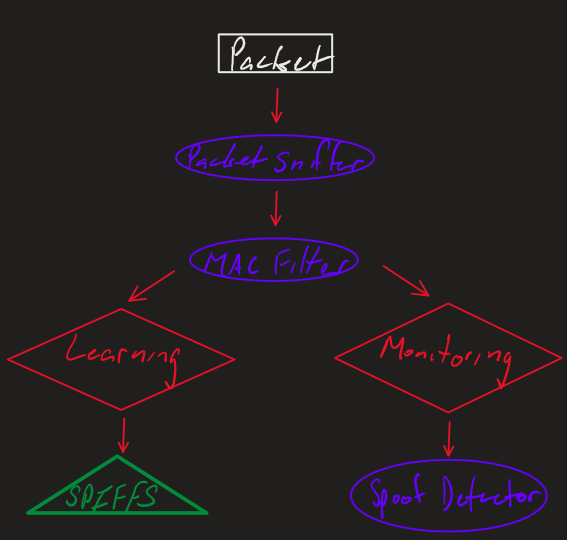
\includegraphics[width=0.8\textwidth]{Diagram.png}
    \caption{System Diagram}
    \label{fig:SystemDiagram}
\end{figure}

The figure above shows a very general overview of how the system works. The ESP32 detects packets in promiscuous mode which are then processed by the Packet Sniffer function. The MAC 
Filter removes packets being sent to or from the other access points on the network and also ignores packets sent to \textbf{\lstinline[]|FF:FF:FF:FF:FF:FF|}, (the broadcast address) to prevent the device from
flooding the storage with unnecessary packets. Depending on what "mode" the device is currently operating in, it will either save the packet information to the 
\textbf{\lstinline[]|known\_connections\_file|} or compare the RSSI of the incoming packet to the RSSI of the other recently received packets to try and determine if it's coming from a 
spoofed MAC address.

\newpage
\vspace{5mm}
\noindent\textbf{Assumptions}

One of the core assumptions that I made on this project was that I could isolate the traffic being sent to the access point that I wanted to target. I assumed that by filtering out the MAC addresses
of the other access points on the network (since it's a shared network for the entire apartment complex), I would be able to get a good idea of the traffic that was being sent to my specific access point.
I unfortunately don't know if this assumption was correct and am unsure of whether I successfully isolated the traffic that was being picked up by the ESP32.
\\\indent Another assumption I made was that the RSSI values of the packets relating to the MAC address of the access point would be consistent enough to distinguish between the 
access point's legitimate traffic and the traffic of a device attempting to spoof the MAC address. As mentioned before, I wanted to use the IP because it would remain consistent regardless of the 
MAC address changing but wasn't able to make it work properly. 
\\\indent Lastly, I also assumed that no one else in the apartment complex would be attempting to spoof their MAC address. Because I'm not sure I successfully isolated the traffic, I have to assume 
that any traffic picked up during the learning phase is legitimate traffic and can be used as a baseline to set the RSSI values for the various devices.

\newpage
\begin{lstlisting}[language=C++, caption=Packet Sniffer and MAC Filter, label=lst:main_code]
// Ignored MACs
const DeviceInfo ignoredMACs[] = {
    { { 0xFF, 0xFF, 0xFF, 0xFF, 0xFF, 0xFF }, 0, 0, 0 }  // Broadcast address
};
// Function to check if a MAC address should be ignored
bool isIgnoredMAC(const uint8_t *mac) {
  // Check against ignored MACs list
  for (const auto &ignored : ignoredMACs) {
    if (memcmp(mac, ignored.mac, 6) == 0) {
      return true;
    }
  }

  // Make sure not to ignore the Host AP's MAC address
  if (mac[0] == 0x84 && mac[1] == 0x23 && mac[2] == 0x88 && mac[3] == 0x7B && mac[4] == 0x90 && mac[5] == 0xA0) { 
    return false;
  } 
  //Ignore the MAC addresses of other APs on network
  else if (mac[0] == 0x84 && mac[1] == 0x23 && mac[2] == 0x88) {
      return true;
  }
  return false;
}

// Packet sniffer function
void sniffer(void *buf, wifi_promiscuous_pkt_type_t type) {
  wifi_promiscuous_pkt_t *packet = (wifi_promiscuous_pkt_t *)buf;
  uint8_t *srcMAC = &packet->payload[10];
  int rssi = packet->rx_ctrl.rssi;

  // Skip ignored MACs
  if (isIgnoredMAC(srcMAC)) return;

  updateObservedDevices(srcMAC, rssi);
  if (learningMode) {
    // Print during active window
    const char *pktType = (type == WIFI_PKT_MGMT) ? "MGMT" : "DATA";
    Serial.printf("%s - MAC: %s RSSI: %d dBm\n", pktType, macToString(srcMAC).c_str(), rssi);
  } else {
    checkForSpoofing(srcMAC, rssi);
  }
}
\end{lstlisting}
The packet sniffer is one of the main functions, and is responsible for detecting the packets that are sent to the access point. After detecting a packet, the function checks if the MAC address
is in the ignored MACs list by calling \textbf{\lstinline[]|isIgnoredMAC|}. The function will check if the MAC address is in the ignored MACs list, and if it is, the ESP32 will ignore the packet 
and move on to the next one. If it isn't, the function will call the \textbf{\lstinline[]|updateObservedDevices|} function to update the list of recently observed devices which are used to compare 
RSSI values. If the device is in learning mode, the function will also print the MAC address and RSSI of the packet to the serial monitor for the user to see, but due to the sheer volume of network 
traffic, the user cannot properly read the information of every packet without pausing the Serial. If the device is in monitoring mode, the function will call \textbf{\lstinline[]|checkForSpoofing|}  
to try and determine if the MAC address is spoofed or not.

\newpage
\begin{lstlisting}[language=C++, caption=Spoof Detection, label=lst:spoof detector]
int AVG_AP_RSSI = 0;
// Check if the AP's MAC was detected during learning mode
void detectAP_MAC() {
  for (const auto &device : knownDevices) {
    if (memcmp(device.mac, AP_BSSID, 6) == 0) {
      foundAPMAC = true;
      break;
    }
  }
  if (foundAPMAC) {
    for (const auto &device : knownDevices) {
      if (memcmp(device.mac, AP_BSSID, 6) == 0) {
        Serial.printf("AP's MAC address: %s was detected during learning mode. RSSI: %d dBm\n", macToString(device.mac).c_str(), device.avgRSSI);
        AVG_AP_RSSI = device.avgRSSI;
        Serial.printf("Average RSSI of AP: %d dBm\n", AVG_AP_RSSI);
        break;
      }
    }
  } else {
    Serial.println("AP's MAC address was NOT detected during learning mode.");
  }
}
// Check for MAC spoofing
void checkForSpoofing(const uint8_t *mac, int rssi) {
  unsigned long currentTime = millis();

  // Check if MAC matches AP's MAC
  if (memcmp(mac, AP_BSSID, 6) == 0) {
    Serial.println("\nALERT: Device using AP's MAC address detected!");
    return;
  }

  // Check against known devices
  for (const auto &known : knownDevices) {
    if (memcmp(mac, known.mac, 6) == 0) {
      if (abs(rssi - known.avgRSSI) > RSSI_VARIATION_THRESHOLD) {
        Serial.printf("\nALERT: Known device %s shows abnormal RSSI change! Current RSSI: %d dBm, Known Avg RSSI: %d dBm", macToString(mac).c_str(), rssi, known.avgRSSI);
        break; // Stop after the first match
      }
      return;
    }
  }

  // Check for MAC randomization
  for (auto &observed : observedDevices) {
    if (abs(rssi - observed.avgRSSI) < RANDOM_MAC_RSSI && memcmp(mac, observed.mac, 6) != 0 && (currentTime - observed.lastSeen) < TIME_WINDOW) {
      if (currentTime - observed.lastAlertTime > TIME_WINDOW) { // Cooldown check
        Serial.printf("\nALERT: Potential MAC randomization detected!");
        Serial.printf("\nCurrent: %s, Previous: %s\n", macToString(mac).c_str(), macToString(observed.mac).c_str());
        observed.lastAlertTime = currentTime; // Update last alert time
        break; // Stop after the first match
\end{lstlisting}

The \textbf{\lstinline[]|checkForSpoofing|} function is the other primary logical function and is responsible for determining if the MAC address is being spoofed or not. It checks for 3 main criteria:
\begin{enumerate}
    \item If the MAC address matches the MAC address of the access point and the RSSI deviates by more than the 20dBm variance threshold
    \item If the RSSI from a known device falls outside of the variation threshold
    \item If the RSSI from an unknown device compared to another recently observed device is within the random MAC RSSI threshold (set to 10 dBm) 
\end{enumerate}
\vspace {2mm}

\indent If any of these criteria are met, the function will print an alert to the serial monitor. During development I tried a few different methods to ensure that the AP's MAC address wasn't ignored and still
allowed a device attempting to spoof the MAC address to be detected. One method I tried using was attempting to pull the IP Source from the IP packet header, but due to my inexperience I couldn't get 
the ESP32 to properly parse the packet header and retrieve the correct information, which lead to the Serial monitor being flooded with incorrect alerts about a device using the AP's MAC address. 
I eventually decided to just use the RSSI as a less effective way to determine if the device was spoofing the MAC address, as if the MAC address stayed the same but the RSSI changed by too much it's 
highly likely that a device is using the AP's MAC address.

\indent After deciding to use the average RSSI, I built the helper function \textbf{\lstinline[]|detectAP_MAC|} in order to store a copy of the access point's average RSSI to a global variable
which is passed into the \textbf{\lstinline[]|checkForSpoofing|} function in the first argument. \textbf{\lstinline[]|detectAP_MAC|} is called at the end of the learning phase to ensure that the 
device properly logs the access point's RSSI and to print the MAC address and RSSI to the serial monitor for the user to review.

\indent The logic behind the third criteria is that if the RSSI of an unknown device is within a 10 dBm range
of another recently observed device, it could be a sign that the device is using a randomized MAC address. The \textbf{\lstinline[]|TIME\_WINDOW|} variable determines how long the observed devices are "kept in memory" 
and is supposed to reset the cooldown period for the alert. However, in testing, it seems that certain devices still manage to trigger the alert more than once within that time period, as shown below, 
likely due to any processing delays that occur when the device is processing the packets. 

\vspace{2mm}
\begin{lstlisting}[language=C++, caption=Serial Output for Spoof Detection, label=lst:spoof detector serial output]
  23:43:38.834 -> ALERT: Potential MAC randomization detected!
  23:43:38.872 -> Current: F6:04:3A:AB:86:9A, Previous: C0:E7:BF:5E:40:C6
  23:43:38.872 -> 
  23:43:38.872 -> ALERT: Potential MAC randomization detected!
  23:43:38.872 -> Current: F6:89:C7:EE:36:30, Previous: 42:86:27:F0:01:AE
\end{lstlisting}
\vspace{2mm}
\indent While not shown here for brevity the background functions, \textbf{\lstinline[]|deleteKnownDevices|}, \textbf{\lstinline[]|saveKnownDevices|}, and \textbf{\lstinline[]|loadKnownDevices|} are used to 
manage the \textbf{\lstinline[]|known\_connections\_file|} JSON file in the ESP32's onboard memory. \textbf{\lstinline[]|deleteKnownDevices|} is toggled during the setup to enable or disable the 
learning mode. \textbf{\lstinline[]|updateObservedDevices|} is used to keep an updated list of any recently observed devices and their RSSI values regardless of whether or not they are in the 
known devices list. While in monitoring mode, \textbf{\lstinline[]|saveKnownDevices|} is called every 60 seconds to update the list of known devices with the most recent RSSI values and any new
devices that were detected in order to keep an accurate baseline for the normal RSSI values.

%---------------------RESULTS---------------------
\newpage
\secHeader{Testing}
\vspace{5mm}
\newline
\indent When testing the device, I would start by letting it enter learning mode and then generate traffic on my computer by frequently pinging the access point and running Spotify in the background.
After the learning period ended, I would then try to trigger the various alerts. The easiest test to trigger an alert was to cover the ESP32 with aluminum foil and paper to introduce some interference
which would then cause a spike in the RSSI values for my computer and trigger an alert. This would also trigger it for other devices, but was occurred less frequently than the alert for my computer 
specifically.

\begin{lstlisting}[language=bash, caption=Testing Known Devices for Abnormal RSSI Values, label=lst:testing]
WINDOWS COMMAND PROMPT:
  Description . . . . . . . . : Realtek 8723DE Wireless LAN 802.11n PCI-E NIC
  Physical Address. . . . . . : 1C-BF-C0-A1-DB-15
  IPv4 Address. . . . . . . . : 172.16.201.160(Preferred)
  Default Gateway . . . . . . : fe80::a55:31ff:feeb:57e5%13
                                172.16.201.1
  DHCP Server . . . . . . . . : 172.16.201.1
  DNS Servers . . . . . . . . : 8.8.8.8
  NetBIOS over Tcpip. . . . . : Enabled

ping 172.16.201.1

Pinging 172.16.201.1 with 32 bytes of data:
Reply from 172.16.201.1: bytes=32 time=5ms TTL=64
Reply from 172.16.201.1: bytes=32 time=6ms TTL=64
Reply from 172.16.201.1: bytes=32 time=8ms TTL=64
Reply from 172.16.201.1: bytes=32 time=5ms TTL=64

Ping statistics for 172.16.201.1:
  Packets: Sent = 4, Received = 4, Lost = 0 (0% loss),
Approximate round trip times in milli-seconds:
  Minimum = 5ms, Maximum = 8ms, Average = 6ms

ARDUINO SERIAL MONITOR:
20:38:04.494 -> Learning complete. Saved 133 known devices.
20:38:04.494 -> Switching to monitoring mode...
20:38:04.494 -> Your MAC address: 1C:BF:C0:A1:DB:15 was detected during learning mode. RSSI: -37 dBm
20:38:04.494 -> AP's MAC address: 84:23:88:7B:90:A0 was detected during learning mode. RSSI: -69 dBm
20:46:18.680 -> ALERT: Known device 78:6D:EB:DF:D5:07 shows abnormal RSSI change! Current RSSI: -80 dBm, Known Avg RSSI: -59 dBm
20:46:29.044 -> ALERT: Known device 1C:BF:C0:A1:DB:15 shows abnormal RSSI change! Current RSSI: -58 dBm, Known Avg RSSI: -36 dBm
20:46:30.222 -> ALERT: Known device CC:95:D7:B1:53:13 shows abnormal RSSI change! Current RSSI: -77 dBm, Known Avg RSSI: -55 dBm
\end{lstlisting}

\newpage
 After testing for changes in the RSSI values of known devices I would then try to trigger the alert for a device using the AP's MAC address by changing the MAC address of my laptop to match the 
 access point's. 
 \begin{lstlisting}[language=bash, caption=Testing AP MAC Address with Large RSSI Variance, label=lst:testing2]
  UBUNTU TERMINAL:
  ubuntu@ubuntu:~$ ip link
  2: wlp1s0: link/ether b8:31:b5:88:34:d9 brd ff:ff:ff:ff:ff:ff
  ubuntu@ubuntu:~$ sudo ip link set wlp1s0 down
  ubuntu@ubuntu:~$ sudo ip link set wlp1s0 address 84:23:88:7b:90:a0
  ubuntu@ubuntu:~$ ip link
  2: wlp1s0: link/ether 84:23:88:7b:90:a0 brd ff:ff:ff:ff:ff:ff 
               permaddr b8:31:b5:88:34:d9
  ubuntu@ubuntu:~$ sudo ip link set wlp1s0 up
  ubuntu@ubuntu:~$ ping 172.16.201.1
  
  ARDUINO SERIAL MONITOR:
  20:51:19.604 -> ALERT: Device using AP's MAC address detected with abnormal RSSI! RSSI: -40 dBm
  \end{lstlisting}


\secHeader{Results}
\vspace{5mm}

The device does work and is capable of properly sniffing packets on the network and is fairly accurate in determining if a device is \textit{potentially} spoofing its MAC address. The reason why
I say potentially is because it can't definitively tell the user that a device is spoofing its MAC address, as it relies purely on the RSSI values of the incoming packets to make its determination. 
Despite this though, there were very few false positives during testing, and any time an alert was displayed on the serial monitor, it was because I was forcing it to trigger the alert. In this context
I'm determining a false positive to be an alert that wa triggered without my intervention. In the span of a 20 minute testing session with a 5 minute learning phase, only 5 alerts were triggered
when I wasn't attempting to trigger them. This largely comes down to natural variance in the RSSI values of the packets that the device was receiving, and with more fine tuning of the RSSI thresholds,
I think I could prevent false positives from occurring at all. However, I'm wary of setting the \textbf{\lstinline[]|RSSI_VARIATION_THRESHOLD|} too low as it would cause the device to become overly
sensitive, and increasing the threshold too high would cause the device to miss out on detecting a spoofed MAC address.
Through my testing sessions, I determined that a natural variance of about 25 seemed to be ideal.

\newpage 
\secHeader{Summary}
\vspace{5mm}

\indent In summary, this project was a solo endeavor that I took in order to learn more about using an ESP32 microcontroller and to experiment with packet sniffing and MAC address spoofing detection.
The device I created operates in two modes: learning and monitoring, and after establishing a baseline for the average RSSI values of the various devices on the network, can accurately determine if a 
device is \textit{potentially} spoofing its MAC address. However, these results rely on the assumption that the average RSSI values determined for the devices during the learning phase are accurate
and that there are no devices on the network that are already trying to spoof their MAC address. While accurate in predicting when a device is spoofing its MAC address, the device still has no way of
definitively determining if a device is spoofing its MAC address or not, and largely relies on the user to interpret the results. 
\\\indent Overall I think the project was a success, and with a little more time I could implement a machine learning algorithm to help the device truly determine if a device is spoofing its MAC address.
Even though it's not perfect, I think the device is a good first step in creating a wireless MAC address spoofing detection system and is a good proof of concept for possible future projects.
\end{document}